%[Tabeller/figurer: figur/tabelltext obligatorisk, textkommentar obligatorisk, glöm inte källhänvisning och numrering, figurtext under figuren, tabelltext över tabellen]
%[Referenser anges enligt IEEE-systemet: i löpande text (i eller efter mening) med siffror i hakparentes, i den ordning de förekommer i texten. Återkommande referenser behåller gamla nummer. Referenslistan kommer sist i dokumentet]

%[Systemet inkl. extrauppgifter beskrivs översiktligt, lämpligen genom figur/er. Bestäm detaljrikedom enligt nuvarande kunskap och lämplighet för figur.]
%[Figurer kommer få revideras under projektets gång.]
%[Det viktigaste är PROCESSEN med att ta fram figuren: "eftersom denna process hjälper gruppen att fokusera tänkandet, att skapa gemensamma tekniska ramar och att rensa bort (en del) tekniska oklarheter."]

% - Lägg in kommentarer här om ni har några idéer eller ser något som borde ändras -

% - Jag använder draw.io för figuren. Går att göra figurer med LaTeX också men det verkar väldigt omständigt -

% - TODO: Ändra ''fönstersensor'' till ''vibrationssensor'' i figuren

\documentclass[a4paper]{article}

\usepackage[swedish]{babel}
\usepackage[T1]{fontenc}
\usepackage[utf8]{inputenc}
\usepackage{graphicx}
\usepackage{array}

\begin{document}
\section*{Systemöversikt}
\label{sec:Systemöversikt}
Larmsystemet är autonomt och består av en uppsättning datoriserade enheter. En persondator ansluts till systemet för att ta emot larmsignal. Systemet består av en centralenhet och ett valbart antal anslutna periferienheter med sensorer av olika typer. Periferienheterna sköter övervakandet av intressanta lägen, så som fönster och dörrar, och skickar larmsignal till centralenheten då de indikerar misstänksam aktivitet. Centralenheten övervakar i sin tur periferienheterna och skickar larmsignal till den anslutna datorn då larm har lösts ut, eller om någon av periferienheterna oväntat kopplas ur. Konfiguration och kalibrering av systemet kan utföras på centralenheten eller genom ansluten dator.
\\

\begin{figure}
	\centering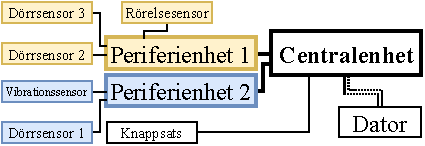
\includegraphics[width=0.8\textwidth]{figurer/systemoversiktfigur1.pdf}
	\caption{Översikt av larmsystemet.}
	\label{figur:översikt}
\end{figure}


I figur \ref{figur:översikt} illustreras ett exempel på en installation av larmsystemet. Det har här installerats i ett hus där \textbf{Periferienhet 2} övervakar huvudingången och hallfönstret, och \textbf{Periferienhet 1} övervakar bakingången, garagedörren och verandan. \textbf{Centralenhetens} knappsats är placerad i anslutning till huvudingången för snabb tillgång till på- och avlarmning.
\\

Systemet har inbyggda säkerhetsmekanismer för att hantera avvikelser. Skulle någon periferienhet eller sensor gå sönder eller oväntat kopplas ifrån så känner centralenheten av detta och skickar larmsignal.

\subsection*{Sensorer}
\begin{description}
\item[Dörrsensorn] är av magnetisk typ och består av två delar, en fästs på dörren och den andra på dörrkarmen. De indikerar när dörren öppnas och magneterna inte längre känner av varandra.
\item[Rörelsesensorn] använder sig av ultraljud för att övervaka ett område, och indikerar när rörelsen i området överstiger ett visst gränsvärde. Gränsvärdet går att ställa in och kalibrera genom centralenheten för att få en lämplig nivå av känslighet.
\item[Vibrationssensorn] är mekanisk och känner av vibration och rörelse\cite{https://www.espruino.com/Vibration}. Den placeras på objektet eller på ett objekt som har direkt fysisk kontakt med objektet. Sensorn indikerar rörelse då den känner av ett värde som överstiger ett gränsvärde. Gränsvärdet ställs in direkt på sensormodulen.
\end{description}

\textbf{}
\end{document}